\setlength\abovedisplayskip{0pt}

\chapter{Ultra-relativistic heavy-ion collisions}

\section{The Standard Model}

The Standard Model describes the fundamental particles of the universe in terms of fermions and bosons. Fermions are particles with half-integer spin, while bosons have integer-spin. This difference in spin has far reaching consequences. Fermions must obey the Pauli Exclusion Principle: only one fermion at a time can occupy a given state. However, multiple bosons can simultaneously occupy a specific state. Subnuclear particles -- protons and neutrons -- contain large numbers of both fermions and bosons. 

Among the fermions are the leptons, neutrinos, and quarks. The leptons consist of the electron, muon, and tau, as well as their anti-particles. The leptons are seemingly fundamental: high energy experiments have yet to observe internal lepton-structure. Neutrinos are weakly interacting particles detected primarily through the precise measuring of missing transverse energy in the products of particle collisions. Quarks are the constituent particles of baryons, which contain three valence quarks, and mesons, which contain two valence quarks. In addition to the valence quarks are the sea quarks, which appear and disappear as quark-antiquark pairs within hadrons. The hadrons are particles made of quarks and gluons. Gluons are particles that mediate the strong nuclear force; likewise, photons mediate the electromagnetic force, and weak-gauge bosons mediate the weak nuclear force. A fourth boson, the graviton, is expected to transmit the gravitational force, but this particles existence has not been verified. 

The behavior of fundamental particles is best described within the framework of quantum field theory (QTF). QFT defines a Lagrangian for fundamental particles. This Lagrangian then predicts the outcome of particle collisions. Different terms in the Lagrangian correspond to the various interactions between particles. The Standard Model Lagrangian, $\mathcal{L}_{Standard Model}$ can be broken down into three basic terms:	
\begin{equation}
\mathcal{L}_{Standard Model} = \mathcal{L}_{QED} + \mathcal{L}_{QCD} + \mathcal{L}_{Higgs} + ... ,  
\end{equation}
Where $\mathcal{L}_{QED}$ is the QED Lagrangin, $\mathcal{L}_{QCD}$ is the QCD Lagrangian, and $\mathcal{L}_{Higgs}$ is the Higgs Lagrangian. The QED and QCD Lagrangians will be the most important in what follows \cite{Halzen:1984mc}. 

The most accessible approach to quantum field theory is through the use of Feynman diagrams. First, one imagines an interaction between particles. Then, one draws this process into a Feynman diagram, which is essentially a pictorial representation of exchanges between particles. The Lagrangian can be interpreted into Feynman rules. These rules describe how the Feynman diagram translates into a calcuation for the quantum mechanical amplitude of the process. The quantum mechanical amplitude, in turn, is proportional to the cross-section of the process. This is important because, sense the cross-section is invariant between experiments, one can use it to effectively test for invariant quantities in the Lagrangian \cite{Peskin:1995ev}.

\section{Quantum electrodynamics}

Quantum electrodynamics (QED) is a theory of electromagnetic interaction in terms of relativistic quantum field theory. QED addresses three specific processes: photon motion, electron motion, and the emission, or absorption, of a photon by an electron. To do this, first a Lagrangian is established based on Maxwell's laws and quantum mechanics. The photon constitutes a spin-1 solution to Maxwell's equations. Likewise, electrons are described, at non-relativistic scales, by the Schrodinger equation, at relativistic scales by the Dirac equation. Figure \ref{fig:qedFeynman} shows the resulting processes allowed by QED: the translation of an electron, the translation of a photon, and the scattering of a photon off an electron \cite{Griffiths:2008zz}.

\begin{figure}[h!]
\begin{centering}
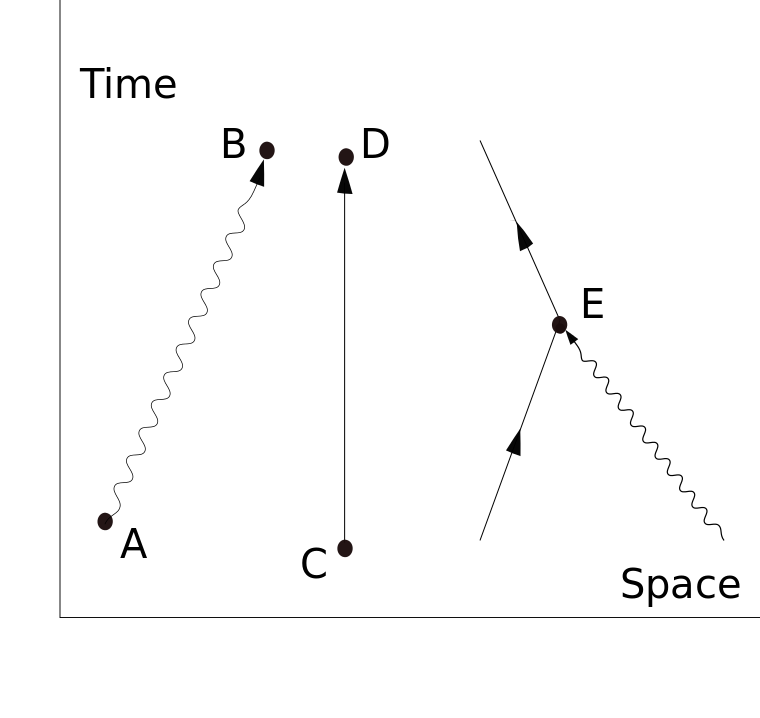
\includegraphics[width=4in]{Chapter1/importfigs/Feynman_Diagram_Components.png}
\par\end{centering}
\caption{QED Components of Feynman Diagrams. \label{fig:qedFeynman}}
\end{figure}

The QED coupling constant, $\alpha_QED$, is approximately ~1/137 at perturbative scales. However, at small scales, i.e. non-perturbative momentum transfers $Q^2$, the coupling constant increases:
\begin{equation}
\alpha_{QED}(Q^2) = \frac{ \alpha_{em}}{(1 - \frac{\alpha_{em}}{3\pi})\mathrm{ln}(\frac{Q^2}{m^2}) },
\end{equation}
where $\alpha_{QED}(Q^2)$ is the QED coupling constant at high $Q^2$, $\alpha_{em}$, and $m$ is the electron mass. High values of $Q^2$ are non-perturbative because, at small scales and high momentum, the fluctuation of photons into electron-positron pairs begins to saturate.

\section{Quantum chromodynamics}

The quarks are a family of fermions that compose the baryons and the mesons. Baryons consist of three quarks in a color neutral state, while mesons consist two quarks in a color neutral state. "Color" in this context refers to the six kinds of strongly-interacting charge available to quarks: red and anti-red, blue and anti-blue, and green and anti-green. Color charge has no relation to optical phenomena, but provides a useful analogy for the stable combinations of quarks. The net color-charge of a baryon or meson is colorless. By way of analogy, a red quark, green quark, and blue quark can together form a hadron, in the way that conventional red, green, and blue can together form white \cite{Brock:1993sz}. 

Gluons are the QCD analogues of the photons in QED. Gluons are spin-1 and massless, but unlike photons, which do not carry electromagnetic charge, gluons carry strongly-interacting charge: color. Color comes six varieties: red, antired, blue, antiblue, green, and antigreen \cite{Wilczek:2000ih}. 

Unlike QED, the QCD coupling increases with distance \cite{Bethke:2006ac}. Figure \ref{fig:runningQCDCoupling} shows the running of the QCD coupling with $Q^2$:
\begin{equation}
\alpha_{QCD}(Q^2) = \frac{4 \pi }{(11 - \frac{2}{3}n_f)\mathrm{ln}(\frac{Q^2}{\Lambda^2_{QCD}}) } ,
\end{equation}
where $n_f$ is the number of quark flavors, $Q^2$ is the momentum transfer, and  $\Lambda^2_{QCD}$ is the mass scale. 
This has the practical consequence of the strong-interactions being stronger in high momentum transfer collisions. The direct results of the running QCD coupling are the dual phenomena of asymptotic freedom and color confinement. At large distances, string tension describes the binding force of the quarks. At short distances, however, Coulomb-like interactions dominate. The QCD coupling constant can be measured via the cross-section of inelastic proton-proton collisions, and also the cross section of electron-positrons into triple jets. 

\begin{figure}[h!]
\begin{centering}
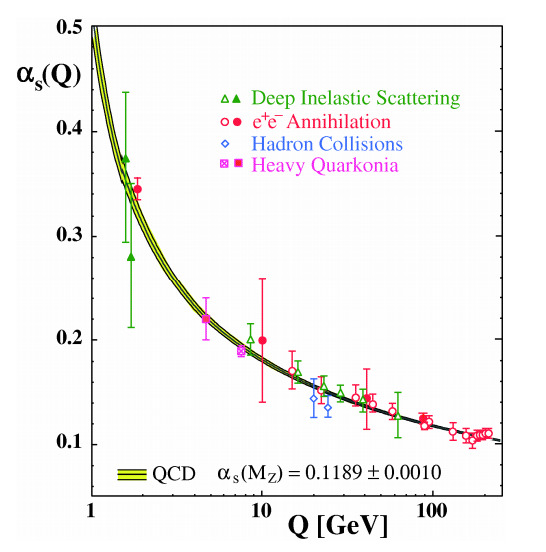
\includegraphics[width=4in]{Chapter1/importfigs/qcd_coupling_bethke.png}
\par\end{centering}
\caption{QCD Coupling Constant vs. $Q^2$. \label{fig:runningQCDCoupling}}
\end{figure}

Within the nucleus, a proton can be thought of as a bubble in a vacuum. Debrye screening exerts a pressure on the proton. This pressure is responsible for the size of the proton. 

\section{QCD experiments}

\subsection{Scattering as a tool}

Scattering experiments are the basic tool for exploring the nucleus. The Large Hadron Collider (LHC) is capable of reaching heavy-ion collision energies of up to 7 TeV per nucleon-nucleon. The higher the energy, the more experiments can probe the nuclear phase-space diagram. Momentum transferred, expressed as $Q^2$, is an important quantity for characterizing QCD measurements. In addition to $Q^2$, Bjorken-x, also known as Bjorken-scaling is necessary to describe the nuclear phase space. Bjorken-x represents the momentum fraction of partons \cite{Bjorken:1968dy}. 

At the turn of the century, Ernst Rutherford probed the gold atom by bombarding a gold sheet with alpha-particles, i.e. helium nuclei. The angular distribution of the scattered alpha-particles demonstrates that the mass of the atom is concentrated in a small volume, i.e, the atom is mostly empty space. Further expedriments revealed that the atomic nuclei consisted of separate positively and neutrally charged particles: protons and neutrons. 

\subsection{Deep inelastic scattering}

Deep inelastic scattering commonly refers to the scattering of a leptons off hadrons. Experiments at HERA focused on electron-proton collisions. In these collisions, the electron was used as a source of photons and neutrinos. When these particles scatter off the proton, the dependence of the collision cross section, on momentum transfer and scattering angle of the source electron, reflects the structure of the proton. These experiments provided the first evidence of two phenomena: the parton model and Bjorken-scaling. 

The parton model, first proposed by Richard Feynman, posits that hadrons in general, and nucleons in specific, are made of more fundamental constituent particles which may or may not be the quarks implied by the SU(3) symmetry. In addition to the quarks, the partons also include any field quanta associated with nuclear forces. In time, these field quanta are dubbed "gluons".

"Scaling" is an interpretation of the data from deep inelastic scattering (DIS). First proposed by James Bjorken, scaling is reflected in the incoherence of photon-proton interactions at photon energies above 1 $GeV/c$. Predictions from perturbative QCD are in good agreement with DIS data from HERA, as seen in figure \ref{fig:qcdBjorkenX}. In this graph the Bjorken-x momentum fraction is designated $x$, and $\sigma_r$ represents the $F_2$ structure function, and $Q^2$ is the transferred momentum from the electron to the proton. The order of magnitude of $\sigma_r$ set by the Bjorken-x.

\begin{figure}[h!]
\begin{centering}
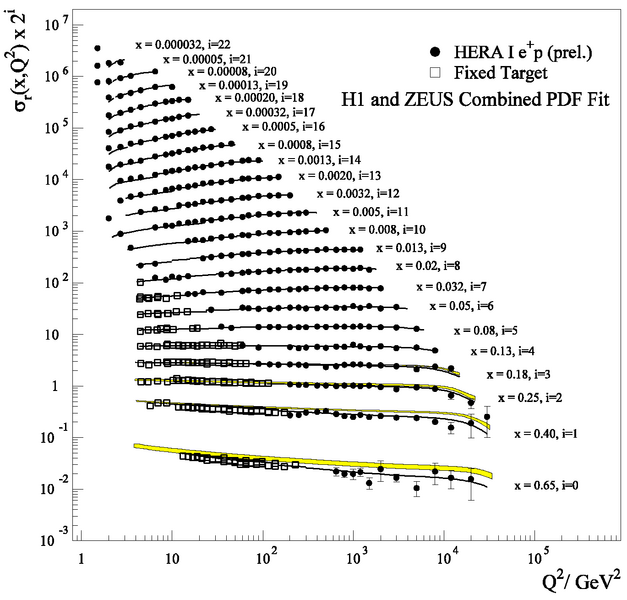
\includegraphics[width=4in]{Chapter1/importfigs/scholarpedia_bjorken_x_qcdExp.png}
\par\end{centering}
\caption{Collision Cross Section vs Bjorken-x, theory and data \cite{Bethke:2006ac}. \label{fig:qcdBjorkenX}}
\end{figure}

At the small scales probed by high energy photons, the decreasing QCD coupling causes quarks and gluons to interact weakly. This phenomena is called "asymptotic freedom". Because gluons themselves carry color charge, the gluons about a quark tend to have an anti-screening behavior: the gluon color adds to the quark color, increasing the net color charge of the area. At smaller distances to a quark, then, there are fewer and fewer gluons augmenting the color interaction.

\subsection{Quark gluon plasma}

The modern understanding of subnuclear physics is based on results from three laboratories: Lawrence Berkeley National Laboratory (LBNL), Brookhaven National Laboratory (BNL), and CERN. Fixed target experiments hinted at the existence of a quark gluon plasma, but the collision energies were too low for this state to last. These experiments confirmed the developing model of the QCD phase space; see figure \ref{fig:QCDPhase}. Essentially, quark matter organizes itself differently depending on temperature and baryon density. At low energies, quark matter exists in bound states: the hadrons. However, in the high energy limit, quarks and gluons take the form of a strongly interacting plasma: the quark-gluon plasma (QGP). The QGP represents the extreme case of asymptotic freedom; the QCD coupling constant becomes small enough that quarks ang gluons no longer behave as bound states. There are two ways of achieving the high energies necessary to form QGP. High baryon densities cause the quarks of separate hadrons to interact at small distances where asymptotic freedom takes effect. It is not currently possible to achive these densities in laboratory experiments, though this state is thought to occur in neutron stars. By contrast, it particle collider's like the LHC increase the energy density by colliding heavy-ions at ultra-relativistic velocities. The high temperature environment thus produced manifests QGP. The early universe, mere milliseconds after the Big Bang, is thought to have existed as QGP. 

\begin{figure}[h!]
\begin{centering}
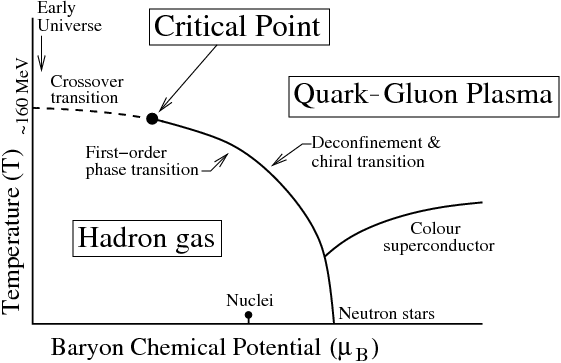
\includegraphics[width=4in]{Chapter1/importfigs/byr13.png}
\par\end{centering}
\caption{QCD Phase Diagram. \label{fig:QCDPhase}}
\end{figure}

There are a number of experimental signatures of QGP. Of particular interest are charm suppression and strangeness enhancement, elliptic flow, jet quenching. The QGP is thought to suppression the production of $J\Psi$ mesons in heavy-ion collisions. The predicted viscosity of QGP would cause elliptic flow in the overlap region of heavy-ion collisions. Lastly, hadronic jets would interact strongly with the QGP; therefore, dijets will have significant energy imbalance depending on the multiple interactions of the components jet with the QGP. All of these cases require a good understanding the heavy-ion initial state as a basis for comparison. 

\section{Parton distribution functions}

Parton distribution functions are a way of encoding hadron data gathered from high energy particle collisions. 

\subsection{Wigner distribution}

One can use the Wigner distribution to tomographically image the internal structure of the nucleus \cite{Hatta:2016dxp}. The nucleus manifests different structures at varying momentum fractions; specifically, small momentum fractions exhibit gluon saturation \cite{Boer:2011fh}; see figure \ref{fig:nuclImag} for an illustration of how the nucleus appears at varying momentum fractions.

\begin{figure}[h!]
\begin{centering}
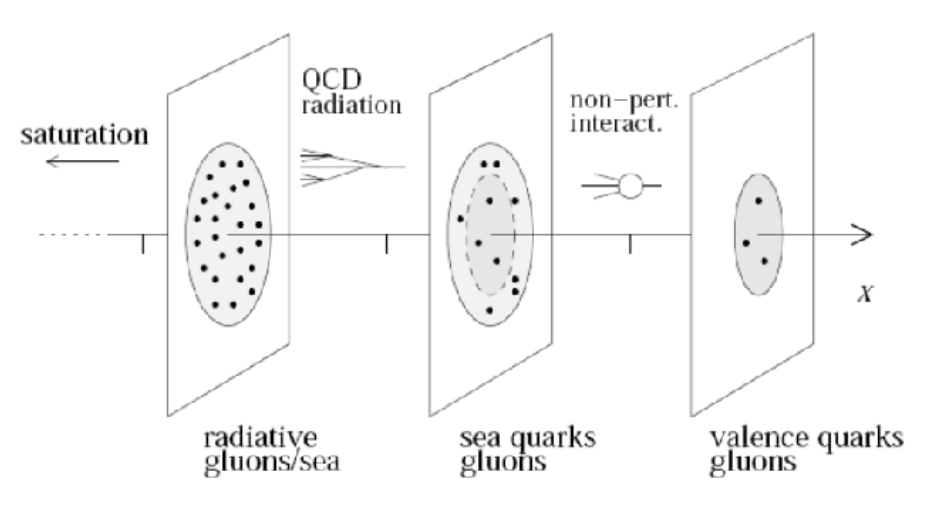
\includegraphics[width=7in]{Chapter1/importfigs/imaging_the_nucleon_upc_dijets_pres.png}
\par\end{centering}
\caption{Subnuclear tomography \label{fig:nuclImag}}
\end{figure}

The quantum field theory lagrangian of the strong interaction is relatively simple, but because of confinement and asymptotic freedom the hadronic bound states are too complex for an analytic solution. Furthermore, collider experiment data requires a quantitative interpretation to be useful. The gap between QCD and heavy-ion data is bridged using the parton model, which considers hadrons as composed of quarks and gluons. Parton density functions (PDFs) model the longitudinal momentum distribution of the partons. PDFs are supplemented by transverse momentum distributions (TMDs) and generalized parton distributions (GPDs). In addition to transverse momentum, GPDs describe the transverse spatial distribution. TMDs and GPDs are derived from the final state particles of a collision. Markus Diehl maps the relationship between various distribution functions in figure \ref{fig:gpdTMDWeb} \cite{Diehl:2003ny}.

The Wigner distribution is a quantum phase space distribution that describes elliptic gluons \cite{Belitsky:2003nz}. Specifically, by considering the color diple scattering amplitude, the angular correlation of the nucleon recoil momentum and the dijet transverse momentum can provide a three-dimensional, tomographic image of the gluons within a high energy nucleus. This tomographic image takes the form of a Wigner distribution, which contains all the information of both TMDs and GPDs without violating the uncertainty principle. Specifically, the angular correlation directly measures the Fourier transform of the gluons. This is possible because the dipole amplitudes are functions of the impact parameter, and because collinear factorization holds. 

\begin{figure}[h!]
\begin{centering}
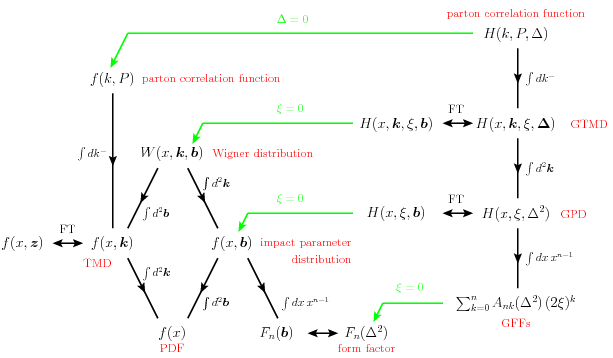
\includegraphics[width=7in]{Chapter1/importfigs/fig6_introGPD_TMD.png}
\par\end{centering}
\caption{Interconnectedness of Parton Distributions. \label{fig:gpdTMDWeb}}
\end{figure}

TMDs and GPDs manifest non-perturbative QCD effects. The Wigner distribution, at this scale, reflects the relationship between the position and momentum of partons. Integrating the Wigner function over the transverse distance yields the TMD, while integrating over transverse momentum yields a GPD with spatial information. 

Yoshitaka Hatta uses the dipole framework to show that the azimuthal angular correlations of coherent dijets are generated by the underlying gluon Wigner distribution. Furthermore, these correlations are consistent with predictions based on standard collinear factorization. Relevant kinematic variables are mapped in the figure \ref{fig:yatta1}.

\begin{figure}[h!]
\begin{centering}
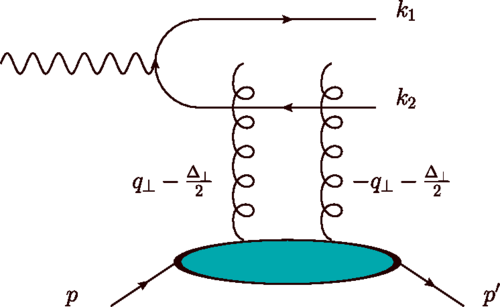
\includegraphics[width=4in]{Chapter1/importfigs/fig4_yatta.png}
\par\end{centering}
\caption{Feynman Diagram of Coherent Dijets in Dipole Framework. \label{fig:yatta1}}.
\end{figure}

It is expected that the dominant contribution to the angular correlation is the ellipitic, corresponding to $n=1$ in the Fourier transform. The interior of the proton displays an intricate structure. 